\documentclass{article}
\usepackage{ismir,amsmath,cite}
\usepackage{amssymb}
\usepackage{graphicx}
\usepackage{color}
\usepackage{framed}
\usepackage{booktabs}

\title{Large-Scale Content-Based Matching of MIDI and Audio Files}

%\twoauthors
%  {Colin Raffel} {LabROSA \\ Department of Electrical Engineering \\ Columbia University \\ New York, NY}
%  {Daniel P. W. Ellis} {LabROSA \\ Department of Electrical Engineering \\ Columbia University \\ New York, NY}

\threeauthors
  {First author} {Affiliation1 \\ {\tt author1@ismir.edu}}
  {Second author} {\bf Retain these fake authors in\\\bf submission to preserve the formatting}
  {Third author} {Affiliation3 \\ {\tt author3@ismir.edu}}

\begin{document}

\maketitle

\begin{abstract}
  MIDI files, when paired with corresponding audio recordings, can be used as ground truth for many music information retrieval tasks.
  We present a system which can efficiently match and align MIDI files to entries in a large corpus of audio content without using any metadata.
  The core of our approach is a neural network-based cross-modality hashing scheme which transforms feature matrices into sequences of vectors in a common Hamming space.
  Once represented in this way, we can efficiently perform large-scale dynamic time warping searches to match MIDI data to audio recordings.
  We evaluate our approach on the task of matching a huge corpus of MIDI files to the Million Song Dataset.
\end{abstract}

\section{Training Data for MIR}\label{sec:introduction}

Central to the task of content-based Music Information Retrieval is the curation of ground-truth data for tasks of interest (e.g. timestamped chord labels for automatic chord estimation, beat positions for beat tracking, prominent melody time series for melody extraction, etc.).
The quantity and quality of this ground-truth is often instrumental in the success of MIR systems which utilize it as training data.
Unfortunately, creating appropriate labels for a recording of a given song by hand typically requires person-hours on the order of the length of the song.
This often arguably makes the available training data a bottleneck to success for a given content-based MIR task.

It has previously been observed that MIDI files, when time-aligned to corresponding audio recordings, can be used to infer ground-truth information about a given song \cite{ewert2012towards, turetsky2003ground}.
This is due to the fact that a MIDI files can be viewed simplistically as a timed sequence of note annotations or a piano roll.
It is much more straightforward to estimate, e.g., beat locations, chord labels, and the predominant melody from these representations than one which was derived from an audio signal.
Unsurprisingly, a handful of tools have been developed for inferring this information from MIDI files \cite{eerola2004mir,mckay2006jsymbolic,cuthbert2010music21,raffel2014pretty_midi}.

In \cite{halevy2009unreasonable}, it is argued that some of the biggest successes in machine learning are thanks to the fact that ``...a large training set of the input-output behavior that we seek to automate is available to us in the wild.''
The main motivation behind this project is that this crucial availability of data holds true for MIDI files - through a large-scale web scrape, we obtained 140,910 unique MIDI files, which is orders of magnitude larger than the datasets typically used for MIR research.
We believe this proliferation of data is largely caused to two factors: First, that karaoke files are typically distributed as MIDI data and that karaoke is wildly popular, and second, that transcribing popular music as MIDI files is a common pastime for hobbyist musicians.

\subsection{Wrangling MIDI files}

The mere existence of a large collection of MIDI data is not enough, however.
As noted above, in order to use MIDI files as ground truth, they need to be both matched (paired with a corresponding audio recording of the same song) and aligned (adjusted so that the timing of the events transcribed in the file match the audio recording).
The latter problem has seen a great deal of research effort \cite{ewert2012towards, turetsky2003ground}, and will not be a main focus of this work.

Given large corpora of audio and MIDI files, the task of matching entries from each may seem to be a trivial problem involving fuzzy text matching of the files' metadata.
However, MIDI files have no formal mechanism for storing metadata (apart from text meta events, which are rarely used), and as a result the best-case scenario is that the artist and song title are included in the filename or subdirectory.
While we found some examples of this in our collection of scraped MIDI files, the vast majority of the files had effectively no metadata information.
Figure \ref{fig:midi-names} shows a random sampling of subdirectory and filenames from our collection.

\begin{figure}
  \begin{framed}
    \scriptsize
    \tt
    J/Jerseygi.mid

    V/VARIA18O.MID

    Carpenters/WeveOnly.mid

    2009 MIDI/handy\char`_man1-D105.mid

    G/Garotos Modernos - Bailanta De Fronteira.mid

    Various Artists/REWINDNAS.MID

    GoldenEarring/Twilight\char`_Zone.mid

    Sure.Polyphone.Midi/Poly 2268.mid

    d/danza3.mid

    100\%sure.polyphone.midi/Fresh.mid

    rogers\char`_kenny/medley.mid

    2009 MIDI/looking\char`_out\char`_my\char`_backdoor3-Bb192.mid
  \end{framed}

  \caption{Random sampling of 12 MIDI filenames and their parent directories from our corpus of 455,333 MIDI files scraped from the Internet.}
  \label{fig:midi-names}
\end{figure}

Fortunately, the goal of matching MIDI and audio files is to find pairs which have \textit{content} in common (i.e., the MIDI file is a transcription of the audio file), an information source which is available regardless of metadata quality.
However, comparing content has the potential to require much more computation than a fuzzy text comparison, and $NM$ comparisons must be made to match a MIDI dataset of size $N$ to an audio file dataset of size $M$.
Motivated by this, we propose a system which can \textit{efficiently} match MIDI files to audio based solely on their content.
Our system learns to hash MIDI and audio content to a common Hamming space where sequences of vectors can be compared efficiently using dynamic time warping (DTW).

The idea of using DTW distance to match MIDI files to audio recordings is not new.
For example, in \cite{hu2003polyphonic}, MIDI-audio matching is done by finding the minimal DTW distance between all pairs of chromagrams of (synthesized) MIDI and audio files.
Our approach differs in a few key ways: First, instead of using chromagrams (a hand-designed representation), we learn a common representation for MIDI and audio data.
Second, our datasets are many orders of magnitude larger (hundreds of thousands vs.\ hundreds of files), which necessitates a much more efficient approach.
Specifically, by mapping to a Hamming space we greatly speed up distance matrix calculation and we receive quadratic speed gains by implicitly downsampling the audio and MIDI feature sequences as part of our learned feature mapping.

In the following section, we detail the dataset of MIDI files we scraped from the Internet and describe how we prepared a subset for training our hasher.
Our cross-modality hashing model is then described in Section \ref{sec:hashing}.
Finally, in section \ref{sec:msd} we evaluate our system's performance on the task of matching files from our MIDI dataset to entries in the Million Song Dataset \cite{bertin2011million}.

\section{Preparing Data}
\label{sec:dataset}

Our project began with a large-scale scrape of MIDI files from the Internet.
We obtained 455,333 files, of which 140,910 were found to have unique MD5 checksums.
Most of these files were transcriptions of pieces of music of varying duration and quality.
As mentioned previously, the majority of these files had very little useful metadata information.
The goal of the present work is to develop an efficient way to match this corpus against the Million Song Dataset (MSD), or more specifically, to the short preview audio recordings provided by 7digital \cite{schindler2012facilitating}.

In order to evaluate our system, we need a collection of MIDI-audio pairs which we know are correctly matched.
The accuracy of our approach can then be judged based on how accurately it is able to recover these pairings using the content of the audio and MIDI files alone.
Fortunately, we identified a subset of files where the subdirectory of the file indicated the artist and the filename indicated the song title.
By cleaning up this subset and using the resulting metadata to match its entries against the Million Song Dataset, we can obtain the requisite ground-truth set of MIDI-audio pairings.
We will refer to this collection of files as the ``clean MIDI subset''.

A further data requirement for our system is a collection of feature vectors derived from audio and MIDI data which should be mapped to similar hashes.
This dataset will be used to train our model for hashing MIDI and audio features to a common Hamming space (described in Section \ref{sec:hashing}).
In our application, we will be matching sequences of hashes using dynamic time warping, so we need to obtain pairs of sequences of feature vectors where the $n$th vector in one sequence should be mapped to the $n$th vector in the other.
This necessitates a collection of MIDI files and audio recordings which we are confident are well-aligned in time.
From this collection, we can extract features for each modality and be sure that there is a direct correspondence between the resulting hash sequences and the original feature vector sequences.

\subsection{Metadata matching}

We first extracted the song title and artist from each entry in the clean MIDI subset based on each MIDI file's filename and subdirectory.
The resulting metadata was still somewhat messy; for example, ``The Beatles'' appeared as an artist along with ``Beatles, The'', ``Beatles'', and ``The Beatles John Paul Ringo George''.
To normalize these issues, we applied some manual text processing and resolved the artists and song titles against the Freebase \cite{bollacker2008freebase} and Echo Nest\footnote{\texttt{http://developer.echonest.com/docs/v4}} databases.
This resulted in 17,243 MIDI files for 10,060 unique songs.

As noted above, we will leverage the clean MIDI subset in two ways: First, to obtain ground-truth pairings of MSD/MIDI matches, and second, to create training data for our hashing scheme.
Note that for the latter purpose, we do not need to restrict ourselves to audio data from the MSD, and we can reasonably expect that by using more training data we may be able to learn a better representation.
As a result, we combined the MSD with three benchmark audio collections: CAL500 \cite{turnbull2007towards}, CAL10k \cite{tingle2010exploring}, and uspop2002 \cite{berenzweig2004large}.
To match these datasets to the clean MIDI subset, we used the Python search engine library Whoosh to perform a fuzzy matching of their metadata.
This resulted in 26,311 audio/MIDI file pairs corresponding to 5,243 unique songs.

\subsection{Synthesized MIDI-to-audio alignment}

Fuzzy metadata matching is not enough to ensure that we have correctly paired MIDI and audio files due to the following potential issues: The metadata could be incorrect, the fuzzy text match could have failed, the MIDI could be a very poor quality transcription (e.g. missing instruments or sections), and/or the MIDI and audio data could correspond to different versions of the same song.
These pitfalls necessitate a method to ensure the correctness of each MIDI/audio file pairing.
In additional, we need to align MIDI files to their corresponding audio recordings to use them as training data for our hashing model.
A common method for performing this kind of alignment is to compute the dynamic time warping (DTW) path between sequences of feature vectors \cite{turetsky2003ground, hu2003polyphonic,ewert2012towards}.
Conveniently, DTW reports a score which represents the quality of the alignment, and unsurprisingly this score tends to be very poor when non-matching sequences are attempted to be aligned.
An overview of DTW and its application to music can be found in \cite{muller2007information}.

For our purposes, the reliability of the DTW confidence score is crucial because we will use it to decide when an audio/MIDI file pairing is valid and when an alignment can be used as training data for our hashing model.
We experimented with a variety of approaches, and converged on the following system for aligning a single MIDI/audio file pair:
First, we synthesize the MIDI data using \texttt{fluidsynth}.\footnote{\texttt{http://www.fluidsynth.org}}
We then estimate the MIDI beat locations using the MIDI file's tempo change information and the method described in \cite{raffel2014pretty_midi}.
To circumvent the common issue where the beat is tracked one-half beat out of phase, we double the BPM until it was at least 240.
Using \texttt{librosa} \cite{mcfee2014librosa}, we compute beat locations for the audio signal with the constraint that the BPM should remain close to the global MIDI tempo. 
We then compute log-amplitude beat-synchronous constant-Q transforms (CQTs) of audio and synthesized MIDI data with semitone frequency spacing and a frequency range from C3 (65.4 Hz) to C7 (1046.5 Hz), also using \texttt{librosa}.
The resulting feature matrices are then of dimensionality $N \times D$ and $M \times D$ where $N$ and $M$ are the resulting number of beats in the MIDI and audio recordings respectively and $D$ is $48$ (the number of semitones between C3 and C7).

\begin{figure*}
  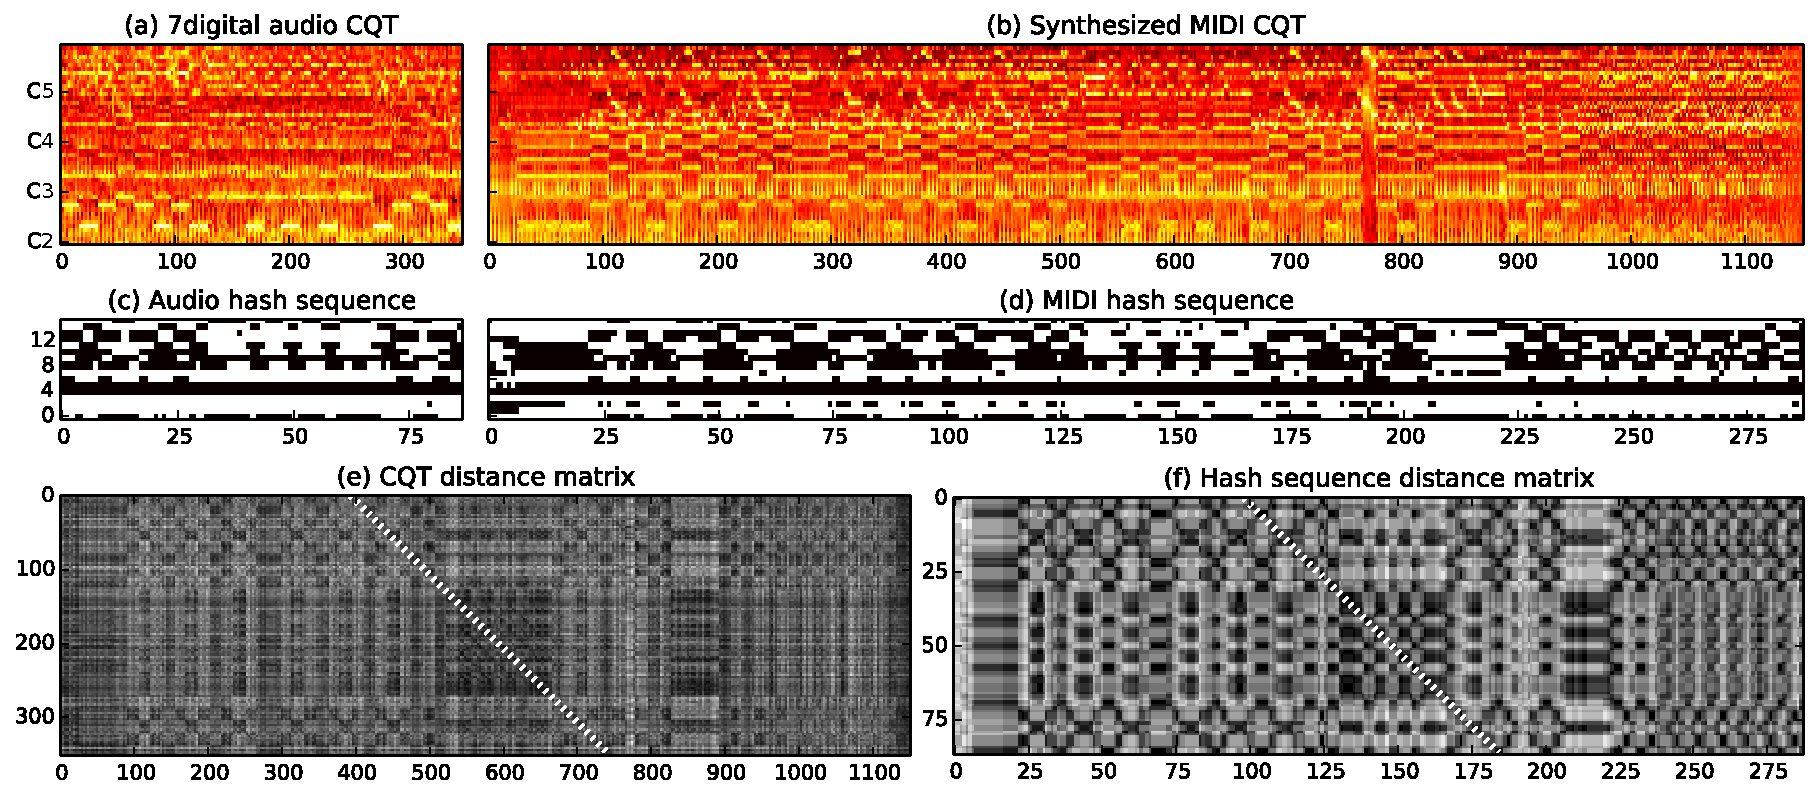
\includegraphics[width=\textwidth]{sims_and_dtws.pdf}
  \caption{Audio and hash-based features and alignment for Billy Idol - ``Dancing With Myself'' (MSD track ID \texttt{TRCZQLG128F427296A}).
           (a) Normalized constant-Q transform of 7digital preview clip, with beat indices and semitones on the horizontal and vertical axes respectively.
	   (b) Normalized CQT for synthesized MIDI file.
	   (c) Hash bitvector sequence for 7digital preview clip, with pooled beat indices and Hamming space dimension on the horizontal and vertical axes respectively.
	   (d) Hash sequence for synthesized MIDI.
	   (e) Similarity matrix and DTW path (displayed as a white dotted line) for CQTs.
	   (f) Similarity matrix and DTW path for hash sequences.}
\end{figure*}

We then use dynamic time warping to find the lowest-cost path through a full pairwise cosine similarity matrix $S \in \mathbb{R}^{N \times M}$ of the MIDI and audio CQTs.
This path can be represented as two sequences $p, q \in \mathbb{R}^L$ of indices from each sequence such that $p[i] = n, q[i] = m$ implies that the $n$th MIDI beat should be aligned to the $m$th audio beat.
Traditional DTW requires that this path includes the start and end of each sequence, or equivalently that $p[1] = q[1] = 1; p[L] = N; q[L] = M$.
This approach is not valid when one sequence may be a subsequence of the other, which is often true in our problem setting due to the fact that, for example, the MSD 7digital audio recordings are cropped preview song clips.
We therefore modify this constraint so that either $gN \le p[L] \le N$ or $gM \le q[L] \le M$ where $g \approx 1$ is a parameter which provides a small amount of additional tolerance.
We also include the typical modification of applying an additive penalty for ``non-diagonal moves'', i.e. path entries where either $p[i] = p[i + 1]$ or $q[i] = q[i + 1]$.
For synthesized MIDI-to-audio alignment, we used $g = .95$ and set the non-diagonal additive penalty to the 90th percentile of $S$.

\subsection{DTW cost as confidence score}

The ``cost'' of a DTW path $p, q$ through $S$ is calculated by the sum of the distances between the aligned entries of each sequence, or
$$
\sum_{i = 1}^L S[p[i], q[i]]
$$
As-is, the DTW cost is not an appropriate confidence score for alignment/match quality in our application primarily for two reasons.
First of all, the path length can vary greatly across MIDI/audio file pairs depending on $N$ and $M$.
We therefore compute the \textit{mean} distance between aligned constant-Q spectra across the path instead of the sum of distances:
$$
\frac{1}{L}\sum_{i = 1}^L S[p[i], q[i]]
$$
Secondly, the scale of $S$ (and therefore the DTW cost) depends on how similar the synthesized audio is to the ``real'' audio recording, which is not an important factor in the alignment quality.
This can be mitigated by normalizing the DTW cost by the mean value of the submatrix of $S$ through which the DTW past travels:
$$
\mathcal{B} = \sum_{i = \min(p)}^{\max(p)} \sum_{j = \min(q)}^{\max(q)} S[i, j] 
$$
These normalizations were also discussed in \cite{hu2003polyphonic}.
Combining the above, we get our modified DTW cost $c$:
$$
c = \frac{1}{L \mathcal{B}} \sum_{i = 1}^L S[p[i], q[i]]
$$
In practice, we found these two normalization steps to be of critical importance for obtaining a reliable confidence score.

In order to use our normalized DTW cost to determine when a match and alignment was successful, we need a threshold above which the DTW cost indicates a failure.
To estimate this threshold, we manually auditioned 125 alignments and noted whether each was successful, where ``success'' requires that the audio and MIDI were well-synchronized for their entire duration.
From this, we obtained an AUROC score of $0.986$, indicating a highly reliable confidence metric.
As a threshold, we chose $0.78$, above which no alignments where labeled as successful.
We discarded all MIDI/audio matches whose alignment resulted in DTW costs above this threshold, resulting in 10,035 successful alignments.

As mentioned above, we will be using these matched and aligned MIDI and audio files for two purposes: First, as training data for our hashing model; and second, to evaluate our efficient content-based matching system.
For fair evaluation, it is critical that we do not test the matching system using any songs which were used to train the hashing model or to adjust the parameters of the matching system.
We therefore split out $50\%$ of the successful alignments to use as training data, $25\%$ as a ``development set'' to tune the content-based matching system, and the remaining $25\%$ to use for final evaluation of our system.
Due to duplication within and across datasets, care was taken to split based on \textit{songs}, rather than by entry.

\section{Cross-Modality Hashing of MIDI and Audio Data}
\label{sec:hashing}

It would be straightforward to use our alignment scheme to match MIDI files with no metadata to entries in a dataset of song recordings.
The size of our entire MIDI dataset (140,910 files) suggests that we should use as large of an audio corpus as possible in hopes that an audio recording of the song corresponding to each MIDI file appears in the corpus.
Towards that end, we will be matching against the Million Song Dataset, the largest standard corpus of popular music recordings.
This necessitates about one million similarity matrix and DTW cost calculations for each MIDI file.
Given the size of our MIDI dataset, if a single MIDI-file-to-audio-dataset matching takes more than a few seconds, matching our entire MIDI dataset would be infeasible.
This means that both computing the similarity matrix and calculating the DTW cost for each MIDI/audio pair must take at most tens of microseconds.

Unfortunately, the method described above does not meet this need.
The median number of beats in the 7digital preview clips from the MSD and the MIDI files are 186 and 1218 respectively.
Computing a cosine similarity matrix of this size (with a feature dimensionality of 48) using the highly optimized C++ code from \texttt{scipy} \cite{jones2014scipy} takes on average 9.82 milliseconds on a Intel Core i7-4930k processor.
When implemented using the LLVM just-in-time compiler Python module \texttt{numba},\footnote{\texttt{http://numba.pydata.org/}} the DTW cost calculation described above takes on average 892 microseconds on the same processor.
It follows that matching a \textit{single} MIDI file to the MSD using this approach would take just under three hours.
Clearly, a more efficient approach is necessary.

Calculating the similarity matrix and the DTW cost are both $\mathcal{O}(NM)$ in complexity.
The fact that computing the similarity matrix takes about 10 times longer is then likely due to the fact that computing each entry in the similarity matrix involves $D$ each of multiply and addition operations.
It follows that calculating the distance between feature vectors is a bottleneck in our system.
In addition, any reduction in the number of feature vectors (beats) in each sequence will give quadratic speed gains for both DTW and similarity matrix calculations.

Motivated by these issues, we propose a system which learns a common representation for the audio and MIDI CQTs in a Hamming space.
By replacing constant-Q spectra with bitvectors, we replace the expensive distance computation with an exclusive-or operation followed by simple table lookup.
This is thanks to the fact that computing the exlcusive-or of two bitvectors $a$ and $b$ will yield a bitvector with $1$s in the dimensions where $a$ and $b$ differ and $0$s elsewhere, and that the number of $1$s in all bitvectors of length $D$ can be precomputed and stored in a table of size $2^D$.
In the course of computing our Hamming space representation, we also implicitly downsample the sequences over time, which provides speedups for both similarity matrix and DTW calculation.
Our approach has the additional potential benefit of learning a representation for comparing audio and MIDI constant-Q spectra, rather than simply using the cosine distance.

\subsection{Hashing with convolutional networks}

Our hashing model is based on the Siamese network architecture proposed in \cite{masci2014multimodal}.
This approach considers the situation where we have feature vectors from two modalities, and two sets $\mathcal{P}$ and $\mathcal{N}$ which contain pairs of feature vectors from each modality such that if $(x, y) \in \mathcal{P}$ then $x$ and $y$ are considered ``similar'' and if $(x, y) \in \mathcal{N}$ they are ``dissimilar''.
A nonlinear mapping is then learned from each modality to a common Hamming space such that similar and dissimilar feature vectors are respectively mapped to bitvectors with small and large Hamming distances.
One possible objective function for this technique is
\begin{align*}
\mathcal{L} &= \frac{1}{|\mathcal{P}|} \sum_{(x, y) \in \mathcal{P}} \| f(x) - g(y) \|_2^2\\
& - \frac{\alpha}{|\mathcal{N}|} \sum_{(x, y) \in \mathcal{N}} \max(0, m - \|f(x) - g(y) \|_2)^2
\end{align*}
where $f$ and $g$ are the nonlinear mappings for each modality, $\alpha$ is a regularization parameter which controls how important it is that the dissimilar pairs be mapped far apart, and $m$ is a threshold above which dissimilar pairs are considered sufficiently distant.

Finding the nonlinear mappings $f$ and $g$ involves optimizing their parameters with respect to $\mathcal{L}$.
The exact form of these nonlinearities is a system design choice; in \cite{masci2014multimodal} they are chosen to be multi-layer nonlinear networks.
In the present work, we will use convolutional networks due to their ability to exploit invariances in the input feature representation.
CQTs contain invariances in both the time and frequency axes, so convolutional networks are particularly well-suited for our task.

In order to apply this technique, we also need to obtain the collections of pairs of similar and dissimilar feature vectors $\mathcal{P}$ and $\mathcal{N}$.
In our problem, our two feature modalities are CQTs from synthesized MIDI files and CQTs from audio files.
We therefore build $\mathcal{P}$ by choosing pairs of constant-Q spectra from simultaneous beats in successfully aligned MIDI/audio pairs.
For example, if $A, B \in \mathbb{R}^{N \times D}$ are CQTs of an aligned MIDI and audio file respectively, then $\mathcal{P}$ will include $(A[1], B[1]), \ldots, (A[N], B[N])$.
The choice of $\mathcal{N}$ is less obvious.
We found that simply randomly choosing CQT spectra from non-aligned beats in our collection of aligned MIDI and audio files achieved satisfactory results.

\subsection{System specifics}

Training our hashing model involves presenting it with training examples and backpropagating the gradient of $\mathcal{L}$ through the model parameters.
Our dataset is the collection of successfully aligned MIDI and audio CQTs described in Section \ref{sec:dataset}.
We split this collection into 90\% train and 10\% validation, where the validation set was not used to optimize the model parameters.
We z-scored the entire training set across feature dimensions and re-used the mean and standard deviation from the training set to z-score the validation set.

For efficiency, we used minibatches of training examples; each minibatch consisted of 50 subsequences, each of of length 100.
These minibatches were extracted by choosing a random offset for each training sequence pair and cropping out a subsequence of length 100.
For $\mathcal{N}$, we simply presented the network with mismatched pairs of subsequences; that is, if $(x, y) \in \mathcal{N}$ then $x$ and $y$ were subsequences from different songs.
Once the network had trained on minibatches from the entire training set (one epoch), we repeated the random sampling process. 
For optimization, we used RMSProp, a recently proposed stochastic optimization technique \cite{tieleman2012lecture}.
Every 100 minibatches, we computed the loss $\mathcal{L}$ on the validation set.
If the validation loss was less than $99\%$ of the previous lowest, we trained for 1000 more iterations (minibatches).

While the validation loss is a reasonable indicator of network performance, its scale will vary depending on the $\alpha$ and $m$ regularization hyperparameters.
To obtain a more consistent metric, we also computed the distribution of distances between the pairs in $\mathcal{P}$ and those in $\mathcal{N}$.
If these distributions are well-separated, we can assume that the network is performing well.
We therefore used the Bhattacharyya distance between these distributions as an alternate performance metric \cite{bhattacharyya1943measure}.

The hashing networks for each modality were chosen to have the same architecture: A series of alternating convolutional and pooling layers followed by a series of fully-connected layers.
All convolutional and fully-connected layers used rectifier nonlinearities except the final output layer, which (as in \cite{masci2014multimodal}) used a hyperbolic tangent nonlinearity.
The first convolutional layer had 16 filters with a filter size of five beats by twelve semitones.
This choice was meant to provide some temporal context and octave invariance.
As advocated by \cite{simonyan2014very}, all subsequent convolutional layers had $2^{n + 3}$ 3x3 filters, where $n$ is the depth of the layer.
All pooling layers performed max-pooling, with a pooling size of 2x2.
Finally, as advocated by \cite{he2015delving}, we initialized all weights with normally distributed random variables with zero mean and a standard deviation of $\sqrt{2/n_{in}}$, where $n_{in}$ is the number of inputs to each layer.
Our model was implemented using Theano \cite{bastien2012theano} and \texttt{lasagne}.\footnote{\texttt{https://github.com/Lasagne/Lasagne}}

To ensure good performance, we optimized all model hyperparameters using Whetlab,\footnote{\texttt{http://www.whetlab.com}} a web API which implements black-box Bayesian optimization \cite{snoek2012practical}.
We used Whetlab to optimize the number of convolutional/pooling layers, the number and size of the fully-connected layers, the RMSProp learning rate and decay parameters, and the $\alpha$ and $m$ regularization parameters of $\mathcal{L}$.
As a hyperparameter optimization objective, we used the Bhattacharyya distance approach described above.
The best performing network found by Whetlab had 2 convolutional layers, 2 ``hidden'' fully-connected layers of with 2048 units in addition to a fully-connected output layer, a learning rate of .001 with a decay parameter of .65, and $\alpha = .5$ and $m = 4$.
This hyperparameter configuration yielded a Bhattacharya distance of $0.488$, indicating a strong separation between distances in $\mathcal{P}$ and distances in $\mathcal{N}$.
\textit{should maybe include a plot here of in-class/out-of-class distribution}

\section{Matching MIDI Files to the MSD}
\label{sec:msd}

Given trained networks, we hash the entire MSD and all MIDIs.
For each MIDI, we compute the DTW distance in the same way as above except that gully = .9 and penalty = 4 and we don't normalize by sim mtx mean.
Because we already matched and aligned, we can look at the rank of the correct match.
We can compute the proportion of matches below a given rank threshold: 1, 13.3\%; 10, 42.3\%, 100, 64.4\%; 1000, 83.3\% - show a plot of this.
We can't solely rely on hash matching, but it can prune out order of magnitude of possibilities with a small loss in accuracy.
We can compute the mean reciprocal rank - .2314.
Most errors caused by incorrect tempo match - show plot of rank vs score with color corresponding to whether the tempo matched.
Speedup: sim mtx is 50-300x faster, DTW is 4-15x faster.
Result: Matching a single MIDI against the MSD takes a few minutes instead of a few hours; parallelized, we are able to match our entire MIDI dataset in 20 days.
Future work: Pruning DTW calculations.

\begin{table}
  \begin{center}
    \begin{tabular}{@{}llllll@{}}
      \toprule
      \textbf{Rank} & 1 & 10 & 100 & 1000 & 10000 \\
      \textbf{Percent $\le$} & 15.2 & 41.6 & 62.8 & 82.7 & 95.9 \\
      \bottomrule
    \end{tabular}
  \end{center}
  \caption{Percentage of MIDI-MSD pairs whose hash sequences had a rank better than each threshold.}
  \label{tab:rank-percentages}
\end{table}

\bibliography{refs}

\end{document}
